% ---------------------------
% Packages and setup

\documentclass[twoside,openright,11pt,a4paper]{report}

\usepackage[utf8]{inputenc}
\usepackage{graphicx}
\usepackage[table,xcdraw]{xcolor}
\usepackage{fullpage}
\usepackage{apacite}
\usepackage{url}
\usepackage{pdfpages}

% stop tables from floating
\usepackage{float}
\restylefloat{table}

\setcounter{secnumdepth}{4}
\usepackage[toc,page]{appendix}

\usepackage{nomencl}
\makenomenclature

\bibliographystyle{apacite}

\graphicspath{ {images/} }

\linespread{1.3}

% make blank pages have "This page is intentionally left blank." on them.

\makeatletter
\def\cleardoublepage{\clearpage\if@twoside%
    \ifodd\c@page\else
    \vspace*{\fill}
    \hfill
    \begin{center}
    This page is intentionally left blank.
    \end{center}
    \vspace{\fill}
    \thispagestyle{plain}
    \newpage
    \if@twocolumn\hbox{}\newpage\fi\fi\fi
}
\makeatother

% ---------------------------

% ---------------------------
% Title page def
\title{\bfseries Free Automated Interconnected Beverage Brewing}
\author{\\\\\\\\\\by Zac Colley\\\\\\\\\\Submitted in partial fulfilment of the requirements for the award of the\\ degree of BSc (Hons) Computer Science of the University of Portsmouth\\\\\\\\\\}
\date{April 2016}
% ---------------------------

% ---------------------------
% Document body
\begin{document}

    \maketitle

    \vspace*{\fill}
  \begin{center}
    \textbf{Preface}\\
    Dedicated to the Jesters and my family
  \end{center}
\vspace*{\fill}
\pagebreak


    \pagebreak
    \tableofcontents
    \raggedbottom

    % Figures and Tables

    \pagebreak
    \listoffigures

    \pagebreak
    \listoftables

    % Nomenclature and Abstract

    \pagebreak
    \printnomenclature

    \pagebreak
    \vspace*{\fill}
  \begin{center}
    \textbf{Abstract}\\
    This abstract should be the last thing you write, it is a summary of the introduction that is only a few sentences long.  At most it should be a couple of paragraphs. It must be very succinct.
  \end{center}
\vspace*{\fill}
\pagebreak

    % Chapters

    \chapter{Introduction} \label{i}

This chapter introduces the overarching themes of this report and places the motivation for the work into context. Thereafter, the rationale and goals defined for the investigation of the project are discussed, followed by a summary of the overall project. Finally, an overview of the dissertation is given on a per-chapter basis.

Your words begin here at the high level, then dive into detail in sections and subsections...

\section{Project Goals} \label{i--project-goals}

The main goal of this project is to create a progressive web application (PWA) through experimentation and implementation of principles such as Performance as User Experience, Offline First and modern web technologies such as Service Workers, Virtual DOM, clientside databases.

\section{Report Outline} \label{i--report-outline}

The rest of this report is organised as follows:

Chapter 1 reviews home-brewing and user experience through performance.

Chapter 2 describes the design of the proposed solution.

Chapter 3 describes the system implementation of the proposed solution and testing.

Chapter 4 is the conclusion with future work.


    \chapter{A Review of Home-brewing and User Experience through Performance} \label{l-r}

\section{Introduction} \label{l-r--introduction}

This first section (\ref{l-r--home-brewing}) of this chapter discusses the current landscape for home-brewing and it's integration with technology. The following section (\ref{l-r--user-experience-performance}) explores the relationship between performance, user experience and modern web development. The analysis and design phase of this project will consider these topics. Finally, section \ref{l-r--summary} summarises the chapter.

\section{Home-brewing} \label{l-r--home-brewing}

Last year, BBPA (The British Beer and Pub Association) estimated pubs in the UK had ``fallen by 19\% since 2000: from 60,800 to 49,433 in 2012". \cite{BBPA}

Craft and independent brewing is on the up however. SIBA (The Society of Independent Brewers), saw an increase of  SIBA’s membership has grown by 49 members in 2015. \cite{SIBA}

Home-brewing, brewing beer on a small personal scale, has been around for thousands of years and has grown popular in the last few years. % citation needed haha

% describe a home brew process?

\subsection{A comparison of home-brewing and OSS} \label{l-r--compare-home-brewing-and-oss}

Sharing recipes, set-ups and brewing techniques is analogous to the open source communities surround software and hardware. Bringing the two together is mutually beneficial.

With the popularity of affordable and accessible computing with platforms such as Raspberry PI and Arduino, introducing computing technologies into home brewing means more automation and control.

Due to the open source nature of these platforms, many systems have been created. One example is BrewPi, a fermentation temperature controller for brewing beer or wine. \cite{brewpi}

This merge of physical creating and software can be seen all across the tech community. One great example is in farming with the MIT Open Agriculture Initiative, ``Every time users grow and harvest, they will contribute to a library of climate recipes that can be borrowed and scaled so that users around the world can gain access to the best and freshest foods.". \cite{climate_recipes}

Ultimately, the Internet is the perfect platform for this type of recipe sharing and collaboration.

\subsection{Existing home-brewing solutions and APIs} \label{l-r--exisiting-home-brewing-solutions}

Data formats have been created to handle brewing recipes and other brewing data, the most mature and popular of which is BeerXML. BeerXML uses the XML format for brewing data. \cite{beerxml} Open and standardized formats in general mean better portability, compatibility for data. % cite?

With a decline in usage of XML, a JSON alternative has been created aptly named BeerJSON. \cite{beerjson} % cite the amount of usage of json over xml

Malt.io is a community website for these brewing recipes. With the options for revision history and `cloning' of recipes it is clear it is inspired by the popular Git repository and social coding network GitHub. \cite{malt.io}

There are many software solutions for various parts of the brewing process. Some of which are reviewed in section \ref{a--d--review-of-existing-software}.

\section{User Experience through Performance} \label{l-r--user-experience-performance}

User experience (referred to as UX), is how a user feels while using a system. There are many aspects to user experience such as usability and accessibility. \cite{what_is_ux}

One of the most important aspects of user experience is the performance. When looking at the web specifically, performance in essence is the perceived speed of websites and the actions taken on them.

When designing and building on the web, performance should be considered at the same level as aesthetics. \cite{performance_is_ux}

\subsection{Speed and Timing} \label{l-r--speed}

There is a lot of research into users' relationship with time.

\cite{usability_engineering} shows time affect how users behave towards a system. A system feels instantaneous with actions taken under 0.1 seconds. Anything over 1 second a user can lose their flow of though on an action. After 10 seconds a users will lose attention and start to multi-task.

In terms of relative time, users percieve faster or slower tasks when there is a difference of 20\% in time. \cite{setting_a_performance_budget}

Google have ``always viewed speed as a competitive advantage", when running experiments by introducing artificial delays into searches ``slowing down the search results page by 100 to 400 milliseconds has a measurable impact on the number of searches per user of -0.2\% to -0.6\%". \cite{speed_matters}

Performance delays aren't merely an annoyance, a bad first impression can result in users not returning. \cite{why_web_performance_matters} confirm that ``88\% of online consumers are less likely to return to a site after a bad experience". Delays are stressful. \cite{ericsson} found that mobile delays are more stressful than standing in line at a shop or even watching a horror movie.

There is a clear demand for performance when looking at the topic of blocking web advertising. A controversial topic as of writing, one of the benefits shown is the increase in performance for users especially on mobile platforms. Typically a browser extension would be used to block adverts. Brave, a browser built with advertisement blocking in from the start claims up to 60\% of page load time is caused by the underlying advertisement technology that loads into various places each time you hit a page on your favorite news site. \cite{brave}

\subsection{Perceived Performance} \label{l-r--perceived-performance}

Before discussing achieving good performance through development aspects, it's worth noting a user is only perceiving this performance. If this perceived performance often can be achieved without technical development.

Optimistic user interfaces (UIs) show a user feedback before the corresponding action has taken place thus giving an excellent perceived performance.

An example of this is the Instagram like button. On press of the like button the application doesn't wait for a round trip to the server to check that action was carried out successfully, instead it shows the user that they have liked the post immediately with the `optimism' that the action will be carried out. \cite{performing_actions_optimisitically}

Lazy-loading is the method of loading content (often images) after initial load for performance. This is often used as part of an optimistic UI.

Using images as an example, having a placeholder based the source image can mean a smoother transition. One technique to achieve this is to create a tiny thumbnail, let the browser resize and then blur to create a gradient based on the image's colour palette. \cite{image_colours_lazy_loading}

% image here

\subsection{Measuring and techniques} \label{l-r--measuring-and-techniques}

Measuring performance is important, data metrics allows for better. Tools such as Google's PageSpeed and WebPageTest give developers metrics across all aspects of web performance. % cite

One metric is SpeedIndex ``is the average time at which visible parts of the page are displayed". The benefit to this metric is it helps measure a usable website over just a loaded website. A website may be usable without all of the content having loaded in. \cite{speed_index}

Best practices include optimising a website's resources and where they are retrieved from. With CSS file growing larger in size [find citation] a emerging approach is through Critical CSS. Serving a part of the CSS on load, loading the rest asynchronously and then caching it all for further visits. \cite{fast_as_heck}

% https://twitter.com/igrigorik/status/706890158323269633
% https://medium.com/google-developers/answers-to-questions-about-performance-9806d2dadfe2#.z973fqsjd
% https://www.filamentgroup.com/lab/mv-initial-load-times.html
% https://twitter.com/aerotwist/status/709668062321098752
% https://www.oreilly.com/ideas/progressive-web-apps-and-whats-next-for-mobile
% https://twitter.com/nolanlawson/status/709480413689937920
% base64 shit
% srcset, picture elemnt thumbnailing

\subsubsection{Performance Budgets} \label{l-r--performance-budgets}

Just like budgeting finances, having a performance budget can give a starting point for working with performance in mind. Having this initial constraint can ensure that performance will be thought of while designing. \cite{performance_budget}

One way to find initial metrics is off of similar websites. As described in section \ref{l-r--speed}, setting the target for the metrics at 20\% will mean users perceive the site as faster.

\subsubsection{Front-end Frameworks and Libraries}

TODO

% https://www.filamentgroup.com/lab/mv-initial-load-times.html
% mvc frameworks and performance \cite{performance_mvc}

\subsubsection{Animation} \label{l-r--animation}

% RAIL, https://www.smashingmagazine.com/2015/10/rail-user-centric-model-performance/ \cite{introducing_RAIL}
% https://aerotwist.com/blog/flip-your-animations/ \cite{FLIP}
% opacity, transform etc
% will-change, edge hack shit. postcss plugin. % https://www.google.com/url?q=https%3A%2F%2Ftwitter.com%2Fhelloanselm%2Fstatus%2F707927523498323969&sa=D&sntz=1&usg=AFQjCNGvTT0uGKWJ0g8FoTN7g9cKKvgI_Q

\subsection{Web typography} \label{l-r--web-type}

Good typography is a great way to improve user experience through usability and accessibility. For example, for some dyslexic users can find incorrectly spaced text hard to read through something called `rivers'. \cite{dyslexia}

Due to the popularity of web fonts it's easy to think this is a quick and easy way to improving the typographical user experience of your website. However, just using a web font alone doesn't guarantee a better typography for users. Web fonts are slow, and if poorly implemented can leave users with no content at all on bad connections. This can create something called `FOIT' (Flash of Invisible Text), in which a browser hides all text that should be styled with a custom font until that font has finished loading. \cite{FOIT}

A great reading experience with default system typefaces is easily achieved. As \cite{against_webfonts} explains: ``Typography is not about aesthetics, it's about serving the text. If even a small percentage of people don't consume your content due to a use of web fonts, your typography is failing."

There are ways to avoid FOIT through progressively applying fonts once they're loaded. These approaches work well for repeat visits to a website as these fonts can then be cached. \cite{FOIT}

\subsection{Serverside} \label{l-r--serverside}

TODO

% streams https://jakearchibald.com/2016/streams-ftw/
% https://www.nginx.com/blog/7-tips-for-faster-http2-performance/
% https://timkadlec.com/2015/02/client-side-templatings-major-bug/

\subsection{Progressive Enchancement} \label{l-r--progressive-enhancement}

TODO

% https://adactio.com/journal/7706
% arguments against progressive enhancement (see tom dale with ember)

\subsection{Offline First} \label{l-r--offline-first}

``Frequently not having any data connection in even the wealthiest and most developed cities of the world has led us to conclude that no, the mobile connectivity/bandwidth issue isn’t just going to solve itself on a global level anywhere in the near future." \cite{hello_to_offline_first}

One of the biggest problems connecting to the Internet across the world is not the availability of devices but the network connections. Every year global mobile broadband subscriptions increases by 25\%. In Q4 2015 there were 21 million in India, 21 million in Africa, 20 million APAC (excluding China and India). By comparison, 5 million Europe and 5 million in North America. \cite{ericsson}

India's biggest e-commerce site Flipkart found 63\% users reaching their mobile site via a 2G network. \cite{flipkart} Developing with a stable and fast network connection in mind is not an option if considering these users.

% bruce's opera talk saying "fuck you for thinking only of the western world"

A offline experience can be progressively enhanced with cached content managed by a Service Worked but even the poorest connection is online. Described by Jake Archibald: ``Lie-Fi is like offline, but it trolls you by pretending to be online. It'll attempt to make a connection for minutes and still fail." \cite{supercharging_page_load}

This uncertainty with network connectivity means an site can never assume a user is completely offline.

Previous methods of caching content was through using Appcache, however the lack of control made it a very dangerous technology to use. % cite

% https://stackoverflow.com/questions/3181080/how-to-detect-online-offline-event-cross-browser

\subsection{Workers} \label{l-r--workers}

When developing on the web historically this meant running client-side Javascript in a single threaded environment. With the introduction of Workers web content can be handled with background tasks.

The two main Workers are Service Workers and Web Workers.

Web Workers create background tasks that can run Javascript that interface back and forth between the main JavaScript tasks. A use case of Web Workers is syncing data between a clientside database and a remote database. \cite{using_web_workers}

Service Workers can be seen more as a proxy server between your server and your main JavaScript thread, the key concept is that of `installing' a Service Worker file to the browser itself registered to a origin. Service Workers are asynchronous and so don't have access to APIs such as XHR.

Some use cases of Service Workers include, caching for a better (and sometimes offline) experience, Push notifications, background data syncing. \cite{service_worker}

\subsection{Performance based projects}

Google have set-up the Accelerated Mobile Pages (AMP) Project as a way to create content optimized for mobile. This project grew from a discussion ``between publishers and technology companies about the need to improve the entire mobile content ecosystem for everyone". AMP is constrained to ensure reliable performance, at the cost of limited flexibility in content. \cite{intro_to_amp}

\section{Summary} \label{l-r--summary}

In Chapter 1 we proposed blah blah blah.

In this chapter the state-of-the-art was categorised into blah (section x) and  blah (section y).  Observations were made on the systems reviewed (section z), and the relevance of the state-of-the-art to blah blah was summarised (section w).

The next chapter presents the design of blah blah, which is a system intended to blah blah.


    \chapter{Artefact Design} \label{a-d}

\section{Introduction} \label{a-d--introduction}

In Chapter 2 we identified that blah blah...
This chapter describes the design of blah blah, a system that blah blah.  First, the chapter describes the project’s design methodology (section 3.2), and system requirements (section 3.3).  A proposed solution is then discussed (section 3.4), followed by a blah blah....


\section{Design Methodology} \label{a-d--methodology}

The design and development of blah blah

\subsection{A Review of Existing Software} \label{a--d--review-of-existing-software}

This section is a review of current home-brewing software.

\subsubsection{BeerSmith}

+ Cross platform (Macintosh, Ubuntu and Windows)

\subsubsection{BeerTools Pro}
\subsubsection{Beer Calculus}
\subsubsection{ProMash}
\subsubsection{BrewPal}
\subsubsection{BrewTarget}
\subsubsection{BeerAlchemy}
\subsubsection{Brewer's Friend}

% Need to review the rest of the brewing software https://homebrew.stackexchange.com/questions/784/what-software-do-most-brewers-use/898]

One thing that is common among all of these choices is their inherent offline nature. As they are installed directly to the computer and not in a web browser.

\subsection{Software Life-cycle Methodology} \label{a-d--methodology--life-cycle}

Choosing a methodology is never one size fits all. Instead considering the environment and team around a project is important. Agile software development offers principles that work well with a team, however there is a lot that can be taken for any project.

Agile development embraces changes in development life-cycle and adapts to them, this is in contrast to traditional plan-driven development in which predictions are used instead. An agile plan is the initial set of goals which will adapt as the project grows. \cite{fowler_agile}

Using an incremental and evolutionary approach is key for this artefact due to it's experimental nature, the goals and proposed solutions will change through-out development.

\subsection{Tools and Services} \label{a-d--methodology--tools}

Kanban boards are a tool to visualise the workflow for a project, an online implementation of this tool is Trello. Trello can be used for multiple scenarios and fits well for a software project. Features, bugs and other research can be represented by cards. \cite{trello} % cite for kanban

Version control is arguably one of the most important tools in software development. It records changes over time so that a previous version of the project can be revisited later. Git is a free and open source distributed version control system that is used on many projects. \cite{git}

While being distributed it's often useful to have a centralized repository, there are many Git repository hosting services. GitHub and Bitbucket are two popular choices. While GitHub encourages Open Source Software on their platform the service itself isn't Open Source. \cite{github} GitLab started as a GitHub clone that is fully Open Source, with the choice to host yourself or use their servers. \cite{gitlab} \cite{bitbucket}

These platforms offer similar features but the artefact will be hosted with GitHub due to the familiarity to the author and also the features it offers.

GitHub has a system of `Issues', which allow for tasks to be tracked. These issues can be commented and then closed when deemed completed. For this project the following labels are used:

\begin{itemize}
  \item \textbf{\colorbox{red}{bug}} - tasks which define a bug in the project
  \item \textbf{\colorbox{blue}{feature}} -  tasks which introduce a new feature to the project
  \item \textbf{\colorbox{yellow}{report}} - tasks which are relevant to the report writing itself
  \item \textbf{\colorbox{green}{greenkeeper}} - a label reserved for the greenkeeper tool (as described in x of this report)
  \item \textbf{wontfix} - tasks that are out of scope and/or outdated and wont be completed
\end{itemize}

Following is a screenshot of the issues at one point in the project:

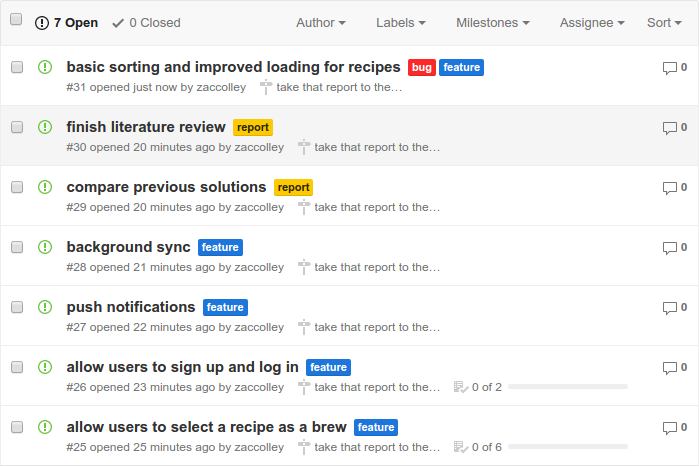
\includegraphics[width=\textwidth,height=\textheight,keepaspectratio]{githubissues}
% have this as a figure?

\section{Requirements} \label{a-d--requirements}

Both the supervisor Rich Boakes and local Portsmouth home-brewer Alan Thompson of GetBrewing.uk, fueled the initial requirements for this project. They saw a need for applications that help improve the current home-brewing ecosystem.

As follows are requirements to create such a application to improve the brewing process when following recipes. After reviewing the current software available in section \ref{a--d--review-of-existing-software} it is clear there are problems in these areas:

\begin{itemize}
  \item Blah
  \item Blah
  \item Blah
  \item Blah
\end{itemize}

One key aspect from a lot of this software is as it is installed to a computer it is offline. Something a traditional web application couldn't achieve. Having the artefact introduce offline features makes for an innovative solution.

This application will look to solve some of these issues.

\subsection{Functional Requirements} \label{a-d--requirements--functional}

The following requirements will be structured through user stories. % cite

\subsubsection{Finding recipes}

\begin{itemize}
  \item As a \textbf{user}, I want to \textbf{search for recipes by recipe and name and description}
  \item As a \textbf{user}, I want to \textbf{browse for recipes by different recipe categories}
\end{itemize}

\subsubsection{Starting a brew}

\begin{itemize}
  \item As a \textbf{user}, I want to \textbf{select and start a brew from any recipe}
\end{itemize}

\subsubsection{Managing a brew}

\begin{itemize}
  \item As a \textbf{user}, I want to \textbf{manage the ingredients for a brew}
  \item As a \textbf{user}, I want to \textbf{be reminded at key stages of a brew}
  \item As a \textbf{user}, I want to \textbf{add notes to key stages of a brew}
  \item As a \textbf{user}, I want to \textbf{review and evaluate the brew on completion}
\end{itemize}

\subsection{Non-Functional Requirements} \label{a-d--requirements--non-functional}

The artefact should:

\begin{itemize}
  \item Follow accessibility guidelines to ensure usage for those of hard of sight
  \item Be documented so that others can maintain
  \item Conform to the performance budget that is set in initial development
  \item Work in specified browser, operating system and screen size environment: x
  \item Pass tests generated throughout and running through continuous integration (such as Travis CI)
\end{itemize}

\section{Proposed Solution} \label{a-d--proposed-solution}

Blah blah blah at a high level, then create subsections that go into detail

\subsection{Performance Budget}

As an initial target for the performance budget we will use a similar website speeds and try and beat them by 20\% (as explained in section \ref{l-r--performance-budgets}).

The chosen website is Malt.io, which has similar functionality to the proposed solution.

\begin{table}[H]
\centering
\begin{tabular}{|l|l|l|l|}
\hline
\textbf{Site}     & \textbf{Start Render} & \textbf{Document Complete} & \textbf{Fully Loaded} \\ \hline
Malt.to           & 2.190s                & 3.998s                     & 4.145s                \\ \hline
Proposed solution & 1.752s                & 3.1984                     & 3.316s                \\ \hline
\end{tabular}
\caption{Performance budget calculation}
\label{table-performance-budget}
\end{table}

The proposed solution will aim to have timings that are equal or below to the results in table \ref{table-performance-budget}.

With performance in mind initially the project will not implement any web fonts or images. The recipes and brew instructions have been determined as the main content and so will be the main focus.

Any iconography will use SVGs for flexibility and overall performance.

\subsection{Data} \label{a-d--data}

This sub-section will describe the gathering data and the storage of said data and creation of data.

\subsubsection{Recipe Gathering}

As noted in section \ref{l-r--exisiting-home-brewing-solutions}, BeerXML is a popular format.
The proposed solution will scrape (process pages using scripts) existing recipe lists for BeerXML recipes.

These files will then be converted into BeerJSON which will be the main recipe format used.

\subsubsection{Databases}

Due to the format of choice BeerJSON, a document store style database that deals directly with JSON documents is a great choice.

There are many document store databases to choose from for example MongoDB, however the chosen database for the proposed solution is CouchDB for it's HTTP API and master-to-master replications. \cite{couchdb}. % cite mongo

The artefact can also make use of PouchDB, a JavaScript database which leverages IndexedDB for clientside databases. PouchDB also has the same API as CouchDB allowing them to sync seamlessly.

An alternative to PouchDB would be localForage. localForage, which also allows for offline databases using IndexedDB , is faster than PouchDB however the syncing feature for PouchDB should outweigh the speed increase here. % cite speed of localforage

\subsection{Technologies} \label{a--d-technologies}

Node.js is a

npm is a package manager for node.js

some packages use epress and passport

% using node with express and passport for data manip and authenication

%  sass, postcss, autoprefixer

% using a virtual dom for dev ergonomics - explore react but other virtudal dom stuff
% jsx, and how it works well with svg too

Due to the artefact's knowledge base around home-brewing, a package called Brauhaus was used. Brauhaus handles conversions of brewing recipes and brewing information. Using this package means that the home-brewing knowledge such as calculations is abstracted away, meaning developers don't necessarily to fully understand the knowledge base to create the application. \cite{brauhaus.js}

% workers

\subsection{Workflow} \label{a--d-workflow}

% atom

% talk about \cite{commitzen}

% talk about linter, babel (es6), snyk

There are many task runners for improving a development workflow such as Gulp, Grunt and Broccoli. A technology that is used in place of task runners for this artefact is Webpack. Webpack bundles all dependencies that you require and indexes them. Webpack knows what dependencies to bundle into your final file where as Gulp and Grunt have to be told which dependencies to bundle through configuration. This results in a smaller file. \cite{webpack}

A smaller file will help for the proposed performance budget and so Webpack will be used. Other technologies such as rollup, which uses `tree-shaking' to achieve a smaller bundle than Webpack can be explored but due to it's infancy this will seen as an experimental implementation. % cite rollup

npm will be used for clientside dependencies. Due to projects such as Browserify which create browser friendly versions of packages it is used for clientside as well as serverside JavaScript. \cite{browserify} Managers such as bower which dedicated itself to front-end dependencies has seen a drop in usage due to this. \cite{bower}

\subsubsection{Continous Integration and Deployment}

As ThoughtWorks describes ``Continuous Integration (CI) is a development practice that requires developers to integrate code into a shared repository several times a day. Each check-in is then verified by an automated build, allowing teams to detect problems early.". \cite{continuous_integration}

There are different ways to achieve CI, the artefact will use Travis CI. Travis CI is a online software-as-a-service CI platform. It allows developers to define a set of tasks to carry out (through a `.travis.yml` file in the repository). These tasks should have a success and fail conditions for Travis to know the status of a build. Examples of tasks include building from dependences, running tests and even miscellaneous tasks such as processing \LaTeX documents. \footnote{This report was created using \LaTeX, a word processing and document markup languages. \cite{latex} This report uses ShareLatex's CI to automatically build the final report PDF when the \LaTeX files are pushed to the GitHub repository. Magic! \cite{sharelatex}}

The deployment will also be triggered by these tests succeeding, ensuring unstable builds of the application are never deployed.

Surge (surge.sh) will being used to deploy, it is command-line tool that allows for simple deployment. Installed through npm, it removes any need for FTP, SSH or other more complicated deployment set-ups. Obviously this has limitations, but for front-end web applications this is a simple and effective option. \cite{surge}

This CI is triggered by pushing to the GitHub repository. This allows for both the code, the tests and deployment to all be together.

\section{Summary} \label{a-d--summary}

This chapter described the high-level requirements and design of a system that blah blah blah.  The chapter started by describing blah.  The proposed solution was then discussed in section blah followed by blah in section blah, etc.
Blah blah is covered in further detail in Chapter 4 which describes the implementation of blah blah.


    \chapter{System Implementation} \label{s-i}

\section{Introduction} \label{s-i--introduction}

This chapter describes how the system was implemented based on teh previous artefact design. From design to implementation a few decisions and technologies changed, first there is discussion of the technologies and data flow in the implemented artefact followed by testing and evaluation of the system.

Figure \ref{figure-application-stack-implementation}, shows the revised application stack for the implementation.

\begin{figure}[H]
  \centering
    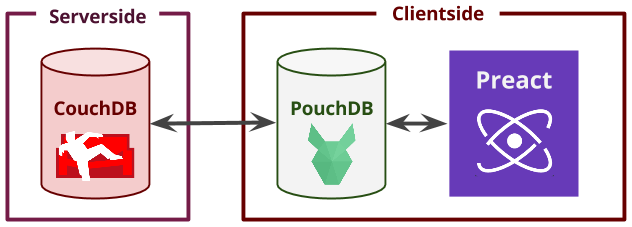
\includegraphics[width=\textwidth,height=\textheight,keepaspectratio]{application_stack_implementation}
  \caption{Overview of how the application stack is structured for the implementation}
  \label{figure-application-stack-implementation}
\end{figure}

The biggest change was the removal of Node.js stack including Express and Passport. As explained fully in section \ref{s-i--data-and-databases} the data manipulation and authentication functionality were handled through CouchDB.

\section{Packages} \label{s-i--packages}

During implementation and research into React and performance another framework was discovered called Preact. Preact, is a framework that attempts to recreate functionality of React but with the focus of performance. Using Preact means a better development experience. \cite{preact} Preact is 3kb in size in comparison to React which is 53kb in size.

The implementation therefore used Preact and was used for rendering views in the artefact.

One principle for software development is DRY (don't repeat yourself). One principle for software development is DRY (don't repeat yourself). ``Every piece of knowledge must have a single, unambiguous, authoritative representation within a system.'' \cite{DRY}

A good example of this is the `moment.js' package used in this artefact, this package handles most date and time related problems. To implement these features is not inherently difficult, but packages such as moment.js offer DRY tried and tested solutions. \cite{moment.js}

\section{Service Worker and Offline Functionality} \label{s-i--sw-offline}

Offline caching of files was implemented through service worker. At the time of writing, there is discussion as to whether service worker is too low level for using the caching functionality. It is argued that this functionality could be brought through as a separate caching API. \cite{sw_sledgehammer}

Implementing the caching with service worker wasn't trivial but once learnt was understandable. Having a abstracted caching API could be useful for simpler implementations of offline caching.

Having a clientside database through PouchDB and IndexedDB (as further discussed in section \ref{s-i--data-and-databases}) not only does this mean offline data but also quick retrieval of data even when connected to a network. This is a boost for performance in general.

\section{Data and Databases} \label{s-i--data-and-databases}

As previously mentioned CouchDB is excellent at master-to-master replication of databases. This means syncing is easily implemented.

The remote database and the local databases sync any changes between themselves, when the local database changes the recipes and brews in state are updated.

In the artefact design data section \ref{a-d--data} and following the decision was to use Node for a Express to handle data coming from the database and Passport to handle user authentication. However through the use of CouchDB and PouchDB it was found that there was no need for either of these technologies.

CouchDB has a user authentication system for handling permission and roles to documents. By default everyone is an admin in what they describe as the `admin party', this is recommended to be disabled but aids development with low barrier to entry when starting a new project.

As the data defines a lot of the structure of the application this authentication system has been leveraged for user authentication for the application.

\section{Interesting Problems} \label{s-i--interesting-problems}

\begin{figure}[H]
  \centering
    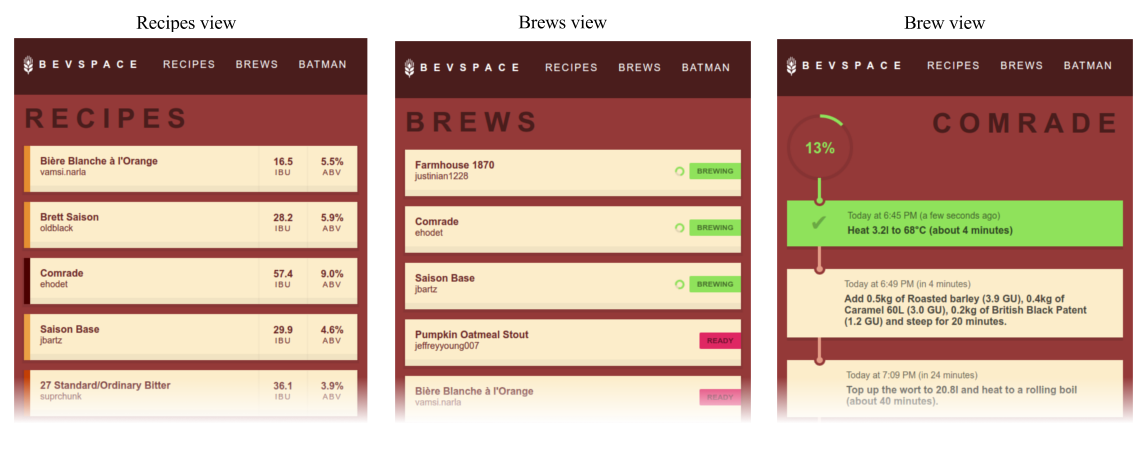
\includegraphics[width=\textwidth,height=\textheight,keepaspectratio]{implementation}
  \caption{Screenshots of different views as implemented}
  \label{figure-implementation-screenshots}
\end{figure}

During the implementation of this project several issues came up. This section discusses some of these issues.

Using newer technologies such as Webpack, ESLint, Babel and Preact come with difficulties. There is a generally a lack of support found online and even some issues can be so new they haven't been documented yet.

For example, with Preact during implementation there was an issue with a feature from React not being supported. This was short-circuit boolean templating, the author then reported this bug which was then fixed. Here having the Preact project as an Open Source project meant this could be fixed not just for this artefact but future users of Preact.

While testing the service worker code and implementation difficulties arise when caching files. Originally the author was manually unregistering the service worker then closing and reopening the tab.

Simply refreshing does not give you any updated version of the service worker files, this is due to the browser making the new page request before unloading the current page so the activated service worker is never released. \cite{refresh_sw}

As shown in Figure \ref{figure-force-update-service-worker}, to solve this problem there is a `Force update on page load' option in the Chrome development tools.

\begin{figure}[H]
  \centering
    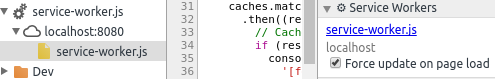
\includegraphics[width=\textwidth,height=\textheight,keepaspectratio]{force_update_service_worker}
  \caption{The `force update on page load' option}
  \label{figure-force-update-service-worker}
\end{figure}

One issue with frameworks and libraries expressed in section \ref{l-r--frameworks} was the lack of control of final code. Having to depend on the Brauhaus package due to a lack of home-brewing knowledge resulted in having to implement more of the library than potentially needed and ultimately a bigger file size reducing performance.

Keeping dependencies up to date is important mostly for security (see Snyk mentioned in section \ref{t-e--testing}), a tool called Greenkeeper (shown in Figure \ref{figure-greenkeeper}) was used through-out which monitors the project's dependencies and sends a Pull Request to the GitHub repository with an updated version of packages. This is great as these Pull Requests can be run through the continuous integration and if it passes the build can be merged straight away. \cite{greenkeeper}

\begin{figure}[H]
  \centering
    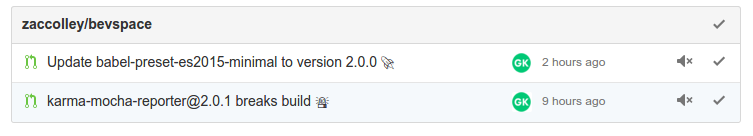
\includegraphics[width=\textwidth,height=\textheight,keepaspectratio]{greenkeeper}
  \caption{Example of Greenkeeper testing different package updates}
  \label{figure-greenkeeper}
\end{figure}

One problem when developing with service workers (and other web APIs) is needed SSL or https when in production. Thankfully, \verb|localhost| is ignored so these features can be used in development easily. Also with projects such as Let's Encrypt, adding SSL to a web site is free and easy. \cite{letsencrypt}

\section{Summary} \label{s-i--summary}

This chapter described the change in technology stack, interesting problems surrounding working with newer technologies such as service worker. It also discusses tools and packages used for the implementation and their benefits.


    \chapter{Conclusion}

\section{Introduction} \label{c--introduction}

In this Chapter, we first summarise the work described in this report (section x). Then we draw a number of conclusions about key parts of the work undertaken in section y, and finally in section z we discuss future work and how we see Semantic Web technologies helping support projects such as this one.


\section{Summary} \label{c--summary}

This is a summary of each chapter  intro and summary
Chapter 1 introduced blah.
Chapter 2 reviewed the state-of-the-art in blah and blah.  Blah was introduced and blah described. The potential for blah blah was highlighted.
Chapter 3 describes the design of blah blah. The separate functions of blah blah that support the requirements were then described in more detail, including blah and blah.
Chapter 4 described the implementation blah blah.
Chapter 5 presented a series of tests that demonstrate blah blah.

\section{Conclusions} \label{c--conclusions}

The aim of this project was to blah blah.  We chose to focus on blah blah.
We then designed and implemented a system that could:
blah
blah
blah
blah
These combined capabilities blah blah blah.
In Chapter 1 we state the general hypothesis that blah blah blah. We have tested this thesis by blah blah.

\section{Key Points} \label{c--key-points}

Discuss future work as you go.

    \subsection{Your key Point}
    Blah point one discussed.
    
    \subsection{Your key Point}
    Your key Point
    Blah point two discussed.


    % References

    \bibliography{references.bib}

    % Appendices

    \begin{appendices}
        \chapter{Project Initiation Document} \label{appendix:pid}

\section{Basic Details}

\begin{table}[h]
\centering
\begin{tabular}{|l|l|}
\hline
Student Name        & Zac Colley                                     \\ \hline
Draft project title & Free Automated Interconnected Beverage Brewing \\ \hline
Course              & Web Technologies                               \\ \hline
Client organisation & GetBrewing.uk                                  \\ \hline
Client contact name & Alan Thompson                                  \\ \hline
Project supervisor  & Rich Boakes                                    \\ \hline
\end{tabular}
\end{table}

\section{Outline of the project environment and problem to be solved}

\textit{In this project I aim to develop a web-based system that will support home-brewers and help to ensure a successful and repeatable brewing process. The system may integrate with brewing hardware and web services in order to provide record and act upon real-time brewing data.}

The project is in partnership with Alan Thompson from GetBrewing.uk, a home brewing company on Elm Grove in Portsmouth.

One of the his products, the Grainfather as a simple control and sensor system. It currently has: a temperature sensor with an LED screen to display this temperature, manual control of the pump and manual control of the heating element.

\textbf{He wishes to offer his brewing kit with an improved control system.}

The proposed solution would improve the Grainfather and help record, collect, share and analyse data amongst brewers.

Apart from the commercial aspect of the project, there is other scientific exploration.

With so many varied set-ups for home brewing, recipes can be tweaked and processes can be changed. The project will explore a web interface to complement the current home-brewing tech eco-system.

\section{Project aim and objectives}

    \subsection{Aims}

        \begin{itemize}
            \item Improve home-brewing processes through design and development of a web application.
            \item There will be a strong focus on user experience research and use of modern development practises.
        \end{itemize}

    \subsection{Objectives}

        \begin{itemize}
            \item Research and apply an designed solution towards a better user experience
            \item Based on UX research, create an intelligent web interface connected to the brewing kit for:
                \begin{itemize}
                    \item Guiding and instructing brewer on current brew
                    \item Recording notes and actions throughout the brew process
                    \item Connecting to current brewing software seamlessly
                \end{itemize}
            \item Analyse user experience approach through structured testing and evaluate the results.
        \end{itemize}

\section{Project deliverables}

Potential deliverables include:

\begin{itemize}
    \item Web interface for a brewing process versioning system
    \item Project report
    \item PID
    \item Trello board
\end{itemize}

\section{Project constraints}

Some of the user interface work would benefit from working on a real-life working brewing kit. While Alan is a contributor to the project, his equipment, specifically the brewing kit is not always accessible for all of the design and development of the web interface. This will mean assumptions must be made and some simulations of the running environment where needed.

\section{Project approach}

I am lacking a lot of knowledge and skills in brewing, this will take some learning. I have contacted other members in the University who have research interests in brewing to learn more.

I am approaching the development with a sprint based model in mind. Simply prioritising which work needs to be tackled in each sprint to reach the goal at hand. This goal may be more research driven or more technically driven depending on the stage of work.

\section{Facilities and resources}

No specialist equipment will be needed from the School of Computing as most of the work can be done on standard PC set-ups.

Research materials from the library will be useful for research.

For the web interface due to the nature of the application of the software it will require real-time technologicals such as an event-driven web scale server (Node.Js) and websockets (through Socket.IO).

Most of the software used will be free to use and so will not require funding. However any of the hardware to interface with the brewing kit would have to be purchased.

\section{Log of risks}

The main risk is the project requires a large amount of hours so any other concerns such as contract work or other course work will lessen the amount of hours.

\textit{\textbf{Risks table goes here}}


\section{Starting point for research}

Through talking to the client more areas of research will be made available.

In terms of the hardware two good places to look are the Open ArdBir and BrewPi projects, both specifically for home brewing.

Finding resources based on user experience in similar areas (machinery, cooking) will make sense.

\section{Breakdown of tasks}

This my initial tasks to start the project:

\begin{itemize}
    \item Research home brewing
        \begin{itemize}
            \item Review previous materials
            \item Talk to Dr Jeremy Mills
        \end{itemize}
    \item Research and choose the technology stack
        \begin{itemize}
            \item For backend versioning system
            \begin{itemize}
                \item Graph databases?
                \item CouchDB
                \item Git
            \end{itemize}
        \end{itemize}
        \begin{itemize}
            \item For the fronted web interface
            \begin{itemize}
                \item React
                \item Node.js (Express, Socket.IO)
            \end{itemize}
        \end{itemize}
\end{itemize}

\section{Project plan}


I will be using Trello to organise my tasks, at each sprint I will work with my supervisor and Alan (where needed) to work out what needs to be put in the sprint. There will also be a backlog of tasks (such as research, development) which will allow a overview of the project easily. This naturally will give an idea of future work for the project too.

\section{Legal, ethical, professional and social issues}

There are no initial pressing legal/ethical/professional/social issues that may impose constraints on the project.

The project has been approved on the ethics website under the same name.

\chapter{Ethics Certificate}

% This is broken on the sharelatex pdf viewer but works on the chrome one (commented part works on built in)
\begin{center}
    % 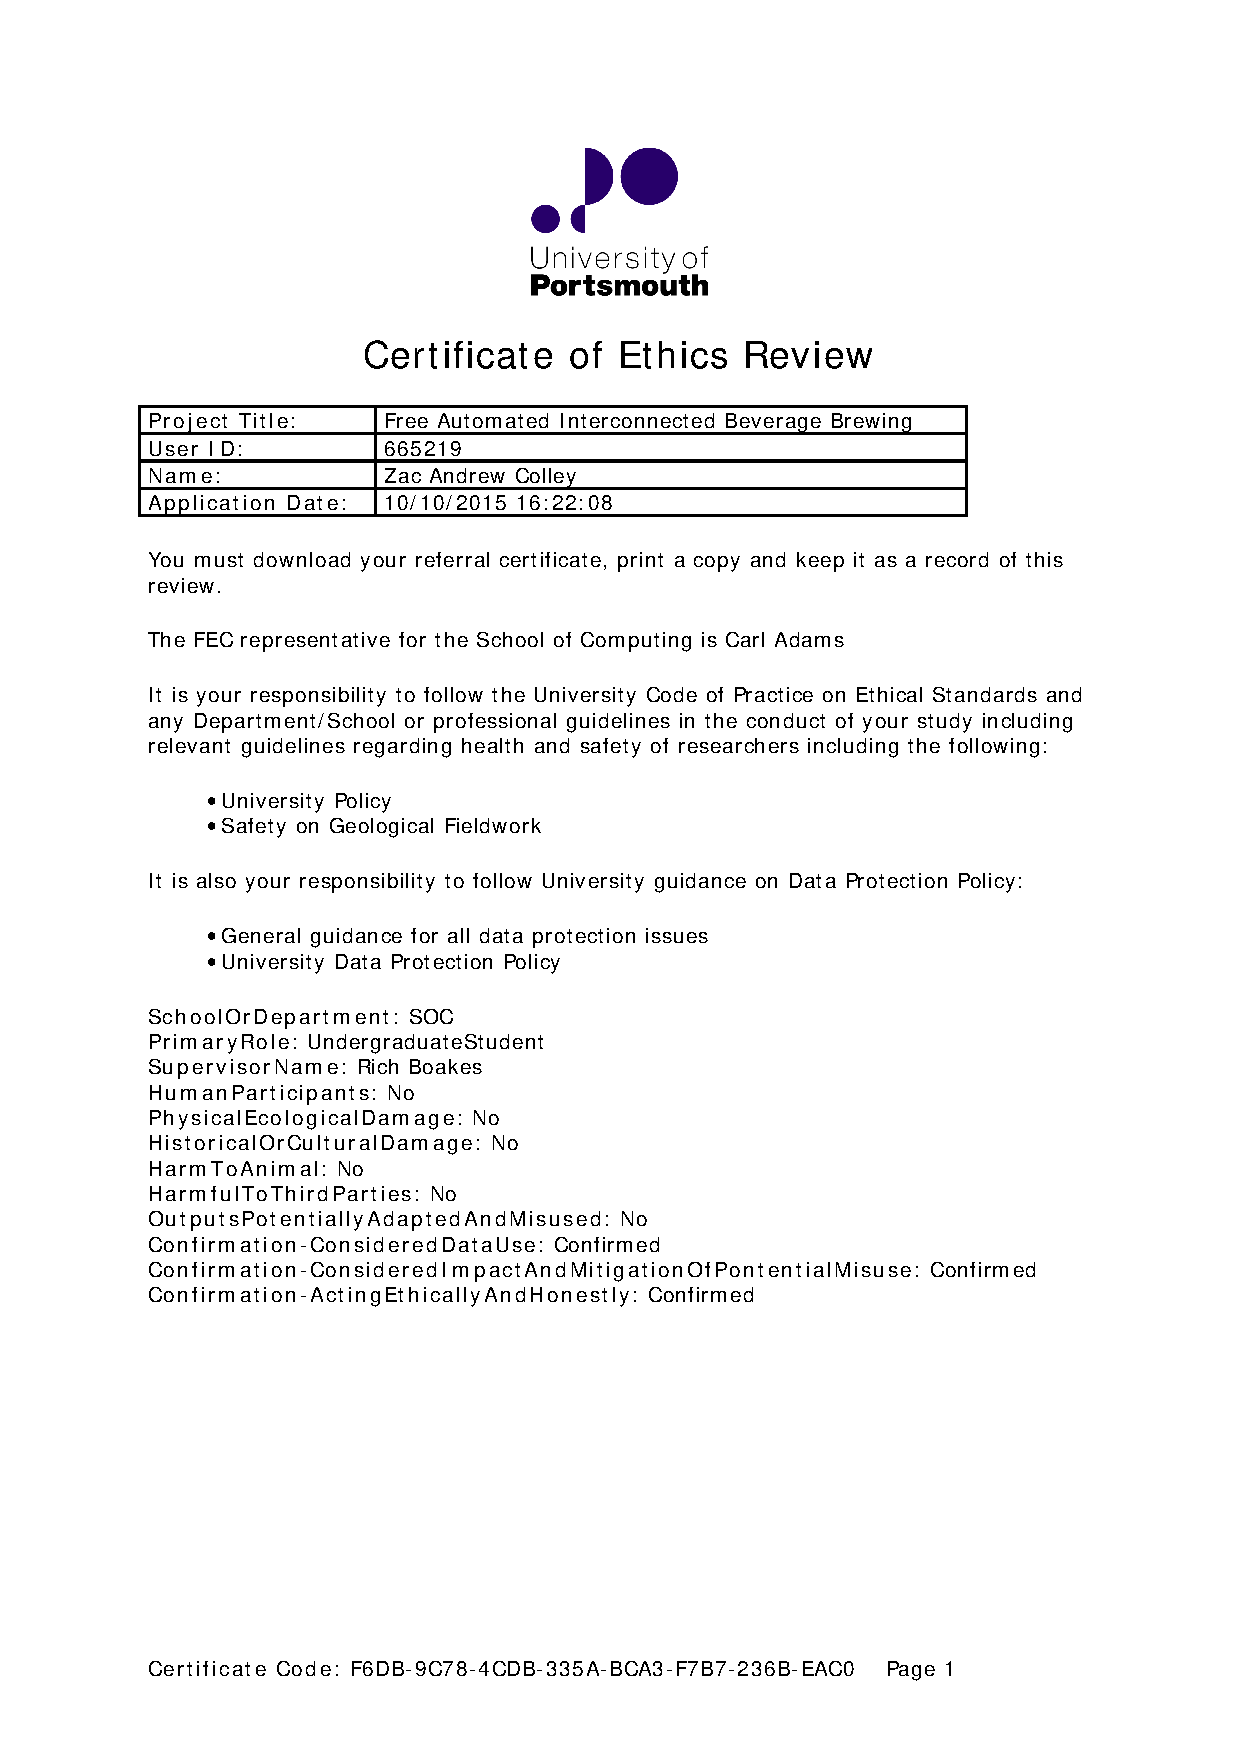
\includepdf[pages=-,scale=1.8,pagecommand={},offset=300 -300]{appendices/ethics-certificate.pdf}
    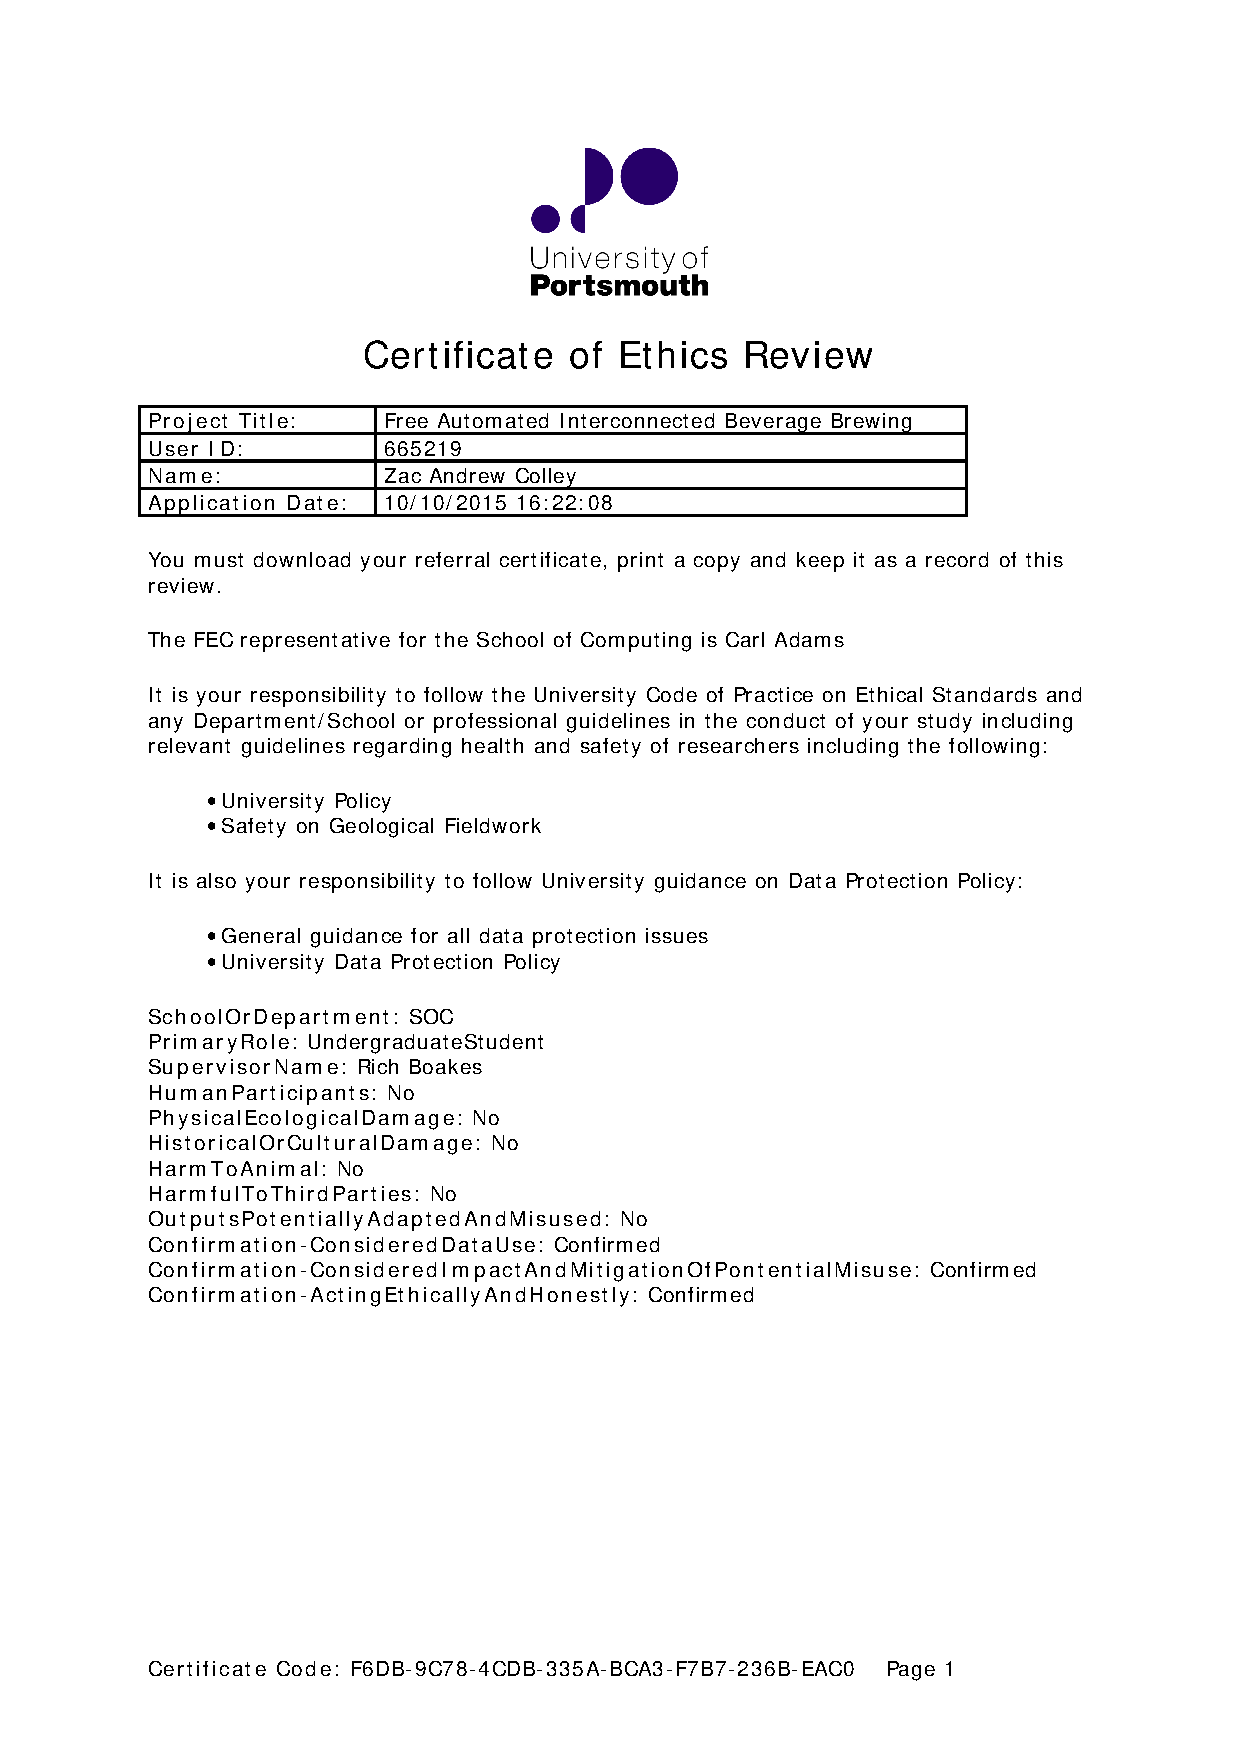
\includepdf[pages=-,pagecommand={},scale=.8,offset=0 50]{appendices/ethics-certificate.pdf}
\end{center}

    \end{appendices}

\end{document}
% ---------------------------
